%!TEX program = xelatex

\documentclass[a4paper, openany, oneside]{memoir}
\usepackage[no-math]{fontspec}
\usepackage{pgfplots}
\pgfplotsset{compat=newest}
\usepackage{commath}
\usepackage{mathtools}
\usepackage{amssymb}
\usepackage{amsthm}
\usepackage{booktabs}
\usepackage{mathtools}
\usepackage{xcolor}
\usepackage[separate-uncertainty=true, per-mode=symbol]{siunitx}
\usepackage[noabbrev, capitalize]{cleveref}
\usepackage{listings}
\usepackage[american inductor, european resistor]{circuitikz}
\usepackage{amsmath}
\usepackage{amsfonts}
\usepackage{ifxetex}
\usepackage[dutch,english]{babel}
\usepackage[backend=bibtexu,texencoding=utf8,bibencoding=utf8,style=ieee,sortlocale=en_GB,language=auto]{biblatex}
\usepackage[strict,autostyle]{csquotes}
\usepackage{parskip}
\usepackage{import}
\usepackage{standalone}
\usepackage{hyperref}
%\usepackage[toc,title,titletoc]{appendix}

\ifxetex{} % Fonts laden in het geval dat je met Xetex compiled
    \usepackage{fontspec}
    \defaultfontfeatures{Ligatures=TeX} % To support LaTeX quoting style
    \setromanfont{Palatino Linotype} % Tover ergens in Font mapje in root.
    \setmonofont{Source Code Pro}
\else % Terug val in standaard pdflatex tool chain. Geen ondersteuning voor OTT fonts
    \usepackage[T1]{fontenc}
    \usepackage[utf8]{inputenc}
\fi
\newcommand{\references}[1]{\begin{flushright}{#1}\end{flushright}}
\renewcommand{\vec}[1]{\boldsymbol{\mathbf{#1}}}
\newcommand{\uvec}[1]{\boldsymbol{\hat{\vec{#1}}}}
\newcommand{\mat}[1]{\boldsymbol{\mathbf{#1}}}
\newcommand{\fasor}[1]{\boldsymbol{\tilde{\vec{#1}}}}
\newcommand{\cmplx}[0]{\mathrm{j}}
\renewcommand{\Re}[0]{\operatorname{Re}}
\newcommand{\Cov}{\operatorname{Cov}}
\newcommand{\Var}{\operatorname{Var}}
\newcommand{\proj}{\operatorname{proj}}
\newcommand{\Perp}{\operatorname{perp}}
\newcommand{\col}{\operatorname{col}}
\newcommand{\rect}{\operatorname{rect}}
\newcommand{\sinc}{\operatorname{sinc}}
\newcommand{\IT}{\operatorname{IT}}
\newcommand{\F}{\mathcal{F}}

\newtheorem{definition}{Definition}
\newtheorem{theorem}{Theorem}


\DeclareSIUnit{\voltampere}{VA} %apparent power
\DeclareSIUnit{\pii}{\ensuremath{\pi}}

\hypersetup{%setup hyperlinks
    colorlinks,
    citecolor=black,
    filecolor=black,
    linkcolor=black,
    urlcolor=black
}

% Example boxes
\usepackage{fancybox}
\usepackage{framed}
\usepackage{adjustbox}
\newenvironment{simpages}%
{\AtBeginEnvironment{itemize}{\parskip=0pt\parsep=0pt\partopsep=0pt}
\def\FrameCommand{\fboxsep=.5\FrameSep\shadowbox}\MakeFramed{\FrameRestore}}%
{\endMakeFramed}

% Impulse train
\DeclareFontFamily{U}{wncy}{}
\DeclareFontShape{U}{wncy}{m}{n}{<->wncyr10}{}
\DeclareSymbolFont{mcy}{U}{wncy}{m}{n}
\DeclareMathSymbol{\Sha}{\mathord}{mcy}{"58}
\addbibresource{../../../includes/bibliography.bib}

\title{Compressive Sensing - An Overview}

\author{W.P. Bruinsma \and R.P. Hes \and H.J.C. Kroep \and T.C. Leliveld \and W.M. Melching \and T.A. aan de Wiel}

\raggedbottom

\begin{document}
\chapter{Software quality \& Testing}
\section{Introduction}
In this chapter we will discuss the methods we used to write a large software product. Traditionally this is not part of a bachelor Electrical Engineering. However we feel the importance of proper code quality is one that every engineer should harness in the ever more software oriented industry. To achieve this we consulted some classic works on the subject. Examples of this are
\begin{itemize}
    \item Code Complete 2: A practical handbook of software construction\cite{mcconnell2004code};
    \item Clean Code: A handbook of agile software craftmanship\cite{martin2008clean};
    \item The Art of Unix Programming \cite{raymond2003art};
    \item Learning Python\cite{lutz2013learning};
    \item Dive into Python\cite{pilgrim2000dive};
    \item Design Patterns: Elements of Reusable Object-oriented Software\cite{designpatterns}.
\end{itemize}
From this the importance of testing became immediately clear. The second is the importance of doing good upfront design. The choice of correct data structures and algorithms makes all the difference. This can be seen in the previous chapters when we refer to design patterns. A third theme is maintainability. This is something that lives through proper documentation and will be discussed below as well. Lastly we wanted to evaluate advice from Code Complete 2, a standard work on code quality, and how this applies to the current state of our software stack.

\section{Testing}
Unit testing is a way of doing verification on code by checking each function with set of known inputs and outputs.

With unit testing you can verify the code on the function level. With the help of special tools you can specify the expectations about the working of a function, in our case the Python \lib{unittest} and \lib{nose} library. Your functions are then run with predefined inputs and the behaviour of the code is then analysed and checked against your specifications.

Unit testing is a great way to easily test if code follows its specifications, and does not break with certain edge cases. Because unit tests run fast, the code can be checked often and mistakes are found early.

For the verification we also used \lib{coverage}. This extension on our unit testing library also keeps track of which lines of code are run during your tests. If certain lines of code are never ran, you know your tests are incomplete. An example of this can be found in \cref{fig:coverage_branch}. In this output a certain branch of an if statement is never taken.

Sometimes it is very easy to write specifications for the correct output of a function. However with certain functions in the reconstructor or the detector, the only way to verify the results was to check them according to known output matrix. These matrices were generated by a \matlab{} script that we assumed was correct\footnote{These \matlab{} scripts were written by the people who were working on the theory}.

*** Hier cijfers over aantal testen en coverage ***

\begin{figure}[h]
    \centering
    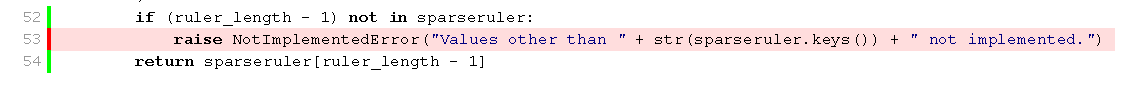
\includegraphics[width=\textwidth]{fig_branch_coverage.pdf}
    \caption{Coverage output of a branch that is never taken}
    \label{fig:coverage_branch}
\end{figure}

\section{Documentation}
\label{sec:documentation}
For the documentation we used Sphinx. Sphinx is a documentation generator that can build a API reference from the docstrings in our code\footnote{A docstring is a comment on the first line of a function indicated with the triple quote}. Sphinx makes use of Python's introspection property which allows it to get all the dosctrings and generate an automated API reference from this. This reference is included with this report.

\section{Qualities of good code}
We will discuss the quality of our code according to the definitions from Code Complete 2 about external and internal characteristics of quality code. External qualities are qualities the user of the software will notice. Internal qualities are only noticed by the developers of the software.\cite{mcconnell2004code}

\subsection{External qualities}
``\textit{Correctness} is the degree to which a system is free from faults in its specification, design, and implementation.'' For our design we used extensive testing to verify the correctness of our code and its results. Our algorithms are base on peer reviewed articles from established authors. This is further confirmed by our automated testing.

``\textit{Usability} is the ease with which users can learn and use a system.'' To easy the adaptability of our system we provide an extensive API documentation of every function of our code. This makes it easy to use the existing functions to expand the system to your own needs.

``\textit{Efficiency} is the minimal use of system resources, including memory and execution time.'' Our design is built with the goal of high performance (see \cref{cha:performance}). While writing the code we thoroughly optimised our program by making use of profiling. We identified bottlenecks and removed them if possible. We also tried to optimise our algorithms and data structures (e.g. using sparse matrices).

``\textit{Reliability} is the ability of a system to perform its required functions under stated conditions whenever required --- having a long mean time between failures.'' From the Art of Unix programming\cite{raymond2003art}: ``The rule of repair: when you must fail, fail noisily and as soon as possible''. In our code we have multiple checks on input data, when the data is not correct it notifies the user and shuts down. With this method we found bugs immediately, and this resulted in very stable system.

``\textit{Integrity} is the degree to which a system prevents unauthorised or improper access to its programs and data. The idea of integrity includes restricting unauthorised user accesses as well ensuring that data is accessed properly --- that is, that tables with parallel data are modified in parallel, that date fields contain only valid dated, and so on.'' When transferring data between different processes we use thread-safe queues, or remote objects. This ensures that no race conditions or other issues with parallel data access can happen. We did not focus on preventing unauthorised access of our data when building this system, this is something that has to be considered when someone else then the user has access to the system.

``\textit{Adaptability} is the extent to which a system can be used, without modification, in applications or environments other than those for which it was specifically designed.'' Because we have written our system in python our code is runnable on all hardware that is supported by Python. This includes all personal computers and even embedded devices with a recent ARM or MIPS processor.

``\textit{Accuracy} is the degree to which a system, as built, is free from error, especially with respect to quantitative outputs. Accuracy differs from correctness; it is a determination of how well a system does the job it's built for rather than whether it was built correctly.'' Before building our system we wrote a specifications for our system. Using testing we can verify that our system adheres to these specifications.

``\textit{Robustness} is the degree to which a system continues to function in the presence of invalid inputs or stressful environmental conditions.'' Our system is not really designed with robustness in mind. However there are multiple fail safes in the system. For example when the sampler does not return the requested number of samples, the frame is discarded and a new one is requested.

\subsection{Internal qualities}
``\textit{Maintainability} is the ease with which you modify a software system to change or add capabilities, improve performance, or correct defect.'' Our system is designed with modularity in mind. All components live in their own module and are not dependent on each other. This makes it very easy to change all small part of the system without interfering with the other parts. By making use of the strategy pattern, different solutions for one problem (e.g. sampling) can be easily added.

``\textit{Flexibility} is the extent to which you can modify a system for uses or environments other than those for which it was specifically designed.'' The system we built is usable for all kinds of high performance signal processing. Instead of samplers, reconstructors and detectors other kind of signal processing modules can be implemented. Also by using the Model-View-Presenter pattern the code is loosely coupled. For example, it is very easy to write another GUI for the system while keeping the other logic intact.

``\textit{Portability} is the ease with which you can modify a system to operate in an environment different from that for which it was specifically designed.'' See \textit{Adaptability}.

``\textit{Reusability} is the extent to which you and the ease with which you can use parts of a system in other systems.'' For all our signal processing blocks we wrote documentation and an API manual. This makes it easy for others to use our modules in their own system.

``\textit{Readability} is the ease with which you can read and understand the source code of a system, especially at the detailed-statement level.'' Our code is written in Python, which is designed to produce very readable code. When our code is not immediately clear to the reader comments are added to improve legibility. Special documentation strings are added to each function to explain the working of each function and explain its arguments.

``\textit{Testability} is the degree to which you can unit-test and system-test a system; the degree to which you can verify that the system meets its requirements.'' Our functional core is almost completely under test. Only the code that interfaces with physical hardware is not testable. The functionality of the reconstruction and the detector is checked with the output of the \matlab{} scripts written by theory group.

``\textit{Understandability} is the ease with which you can comprehend a system at both the system-organisational and detailed-statement levels. Understandability has to do with the coherence of the system at a more general level than readability does.'' By using proven design patterns (Model-View-Presenter) to design our system architecture our system becomes more comprehensible. By separating parts of the system it becomes much easier to reason about a piece of code and its working.




% \subsection{External qualities}
% \begin{description}
% \item[Correctness] The degree to which a system is free from faults in its specification, design, and implementation.
% \item[Usability] The ease with which users can learn and use a system.
% \item[Efficiency] Minimal use of system resources, including memory and execution time.
% \item[Reliability] The ability of a system to perform its required functions under state conditions whenever required --- having a long mean time between failures.
% \item[Integrity] The degree to which a system prevents unauthorised or improper access to its programs and data. The idea of integrity includes restricting unauthorised user accesses as well ensuring that data is accessed properly --- that is, that tables with parallel data are modified in parallel, that date fields contain only valid dated, and so on.
% \item[Adaptability] The extent to which a system can be used, without modification, in applications or environments other than those for which it was specifically designed.
% \item[Accuracy] The degree to which a system, as built, is free from error, especially with respect to quantitative outputs. Accuracy differs from correctness; it is a determination of how well a system does the job it's built for rather than whether it was built correctly.
% \item[Robustness] The degree to which a system continues to function in the presence of invalid inputs or stressful environmental conditions.
% \end{description}

% \subsection{Internal qualities}
% \begin{description}
% \item[Maintainability] The ease with which you modify a software system to change or add capabilities, improve performance, or correct defect.
% \item[Flexibility] The extent to which you can modify a system for uses or environments other than those for which it was specifically designed.
% \item[Portability] The ease with which you can modify a system to operate in an environment different from that for which it was specifically designed.
% \item[Reusability] The extent to which you and the ease with which you can use parts of a system in other systems.
% \item[Readability] The ease with which you can read and understand the source code of a system, especially at the detailed-statement level.
% \item[Testability] The degree to which you can unit-test and system-test a system; the degree to which you can verify that the system meets its requirements.
% \item[Understandability] The ease with which you can comprehend a system at both the system-organisational and detailed-statement levels. Understandability has to do with the coherence of the system at a more general level than readability does.
% \end{description}

\end{document}
